% Installation chapter
You should have by now obtained the latest version of Ubuntu as described in chapter \ref{sect:obtain_ubuntu}. Its now time to try out Ubuntu on your system. If you have not installed an operating system before, do not worry since installing Ubuntu is extremely easy. The sections in this chapter are divided according to different case scenarios. This represents the first step in your journey into the world of Ubuntu. Let's try to make it as smooth as possible. Make sure to read this chapter carefully without skipping ahead.

\section{Prerequisite Steps}
Before proceeding to installing Ubuntu or any other operating system for that matter, it is necessary to make sure the following check list is complete. 

\subsection*{Check if your computer meets the minimum system requirements}
This is one thing which is often overlooked. The minimum system requirement to run Ubuntu with enough room to be comfortable are listed below. The best way to check is try out the Ubuntu Live CD. This is explained in section \ref{sect:live-ubuntu}.

\begin{itemize}
	\item 1 GHz CPU 
	\item 1 GiB Ram
	\item 15 GB Hard Disk Space
	\item 800 x 600 screen resolution
	\item Either a CD/DVD drive or USB port for the installation media
	\item Internet Connection
\end{itemize}

\subsection*{Know how to access your computer's BIOS}
It is necessary to know how to access your computer's BIOS. The BIOS decides which device to boot first. By default, it is set to boot from your hard disk since your current operating system is installed on your hard disk. However, since you are trying out a new operating system, you need to make the boot loader to boot from the CD first. \\

\par \noindent In order to access the BIOS setup, it is required to press a specific keyboard key. The keyboard key required to access your BIOS depends on your computer. You can check \textit{Appendix C} for the keyboard key you need to press for your system. If your computer isn't listed, then you need to search for it online. Once you are in the BIOS setup, choose the CD or USB option and press enter.

\subsection*{Backup your data}
It is always recommended to back up all your personal data onto a separate external storage device as a backup. This is an important and crucial step to avoid loss of personal data in the case of an emergency.

\newpage
\section{Trying out Ubuntu Live} \label{sect:live-ubuntu}
At this point, you may or may not have made your mind about installing Ubuntu permanently to your system. You do not have to install Ubuntu in order to try it out on your system. You can try out Ubuntu using the Live CD option which lets you run Ubuntu on your system without actually installing anything. This is helpful in trying out if Ubuntu works smoothly on your system and to experience Ubuntu before installing it. \\

\par \noindent Follow the steps below to try out Ubuntu using the Live CD option, \\

\par \noindent 1. Insert the Ubuntu installation CD into your CD-ROM. \\

\par \noindent 2. Power on your computer. You need to access the BIOS setup to make the computer to boot from your CD rather than the hard disk.  \\

\par \noindent 3. On booting your computer you are presented with the screen as shown in figure \ref{fig:start-up} . If you do not see this, then your computer is still booting from the hard disk rather than the CD. \\

\begin{figure}[h!]	
	\begin{center}
	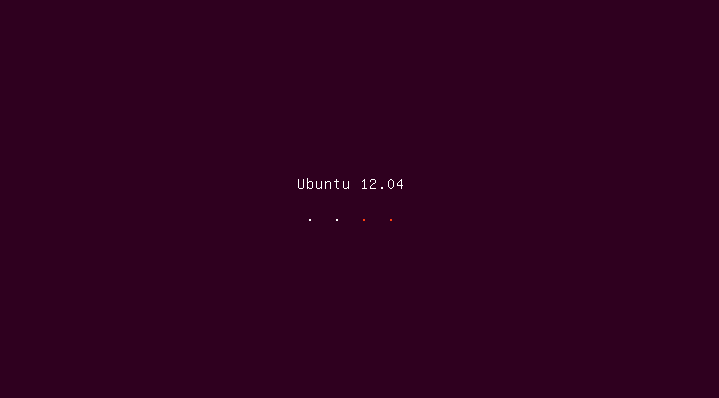
\includegraphics[width=300pt]{./images/installation/basic-start.png}
	\caption{Ubuntu start up screen}	
	\label{fig:start-up}	
	\end{center}
\end{figure}

\par \noindent 4. Wait for Ubuntu to start up. Once the loading is complete, you are presented with the dialogue box as shown in figure \ref{fig:live-options} where you can choose to Try Ubuntu first without installing anything.\\

\begin{figure}[!h]	
	\begin{center}
	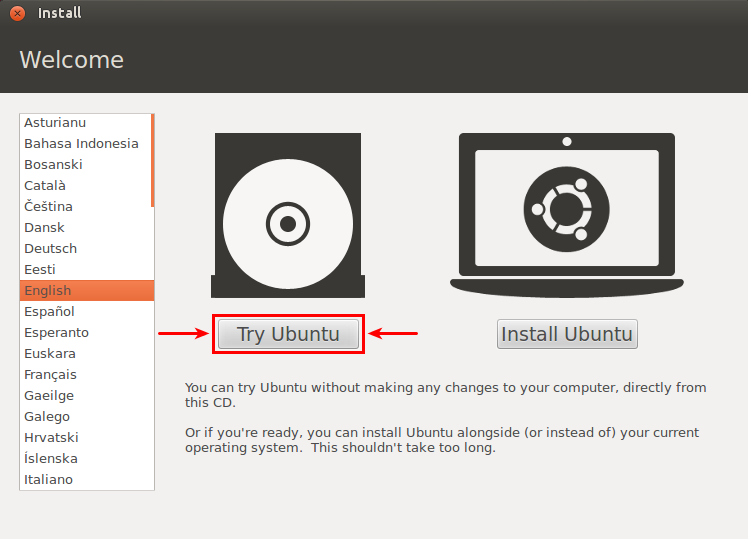
\includegraphics[width=300pt]{./images/installation/install-live-start.png}
	\caption{Try Ubuntu option}	
	\label{fig:live-options}	
	\end{center}
\end{figure}

\newpage
\par \noindent On choosing the "Try Ubuntu" option, you are presented with the Ubuntu desktop as shown in figure. You can use Ubuntu to test out its features to your liking. You can browser the web, check your email and launch applications. If you like what you are using, you can choose to install it permanently by clicking on the Install Ubuntu 12.04 icon present on the desktop. It has been highlighted in figure \ref{fig:live-desktop}. The various installing steps are described in details in the following sections. \\

\begin{figure}[h!]	
	\begin{center}
	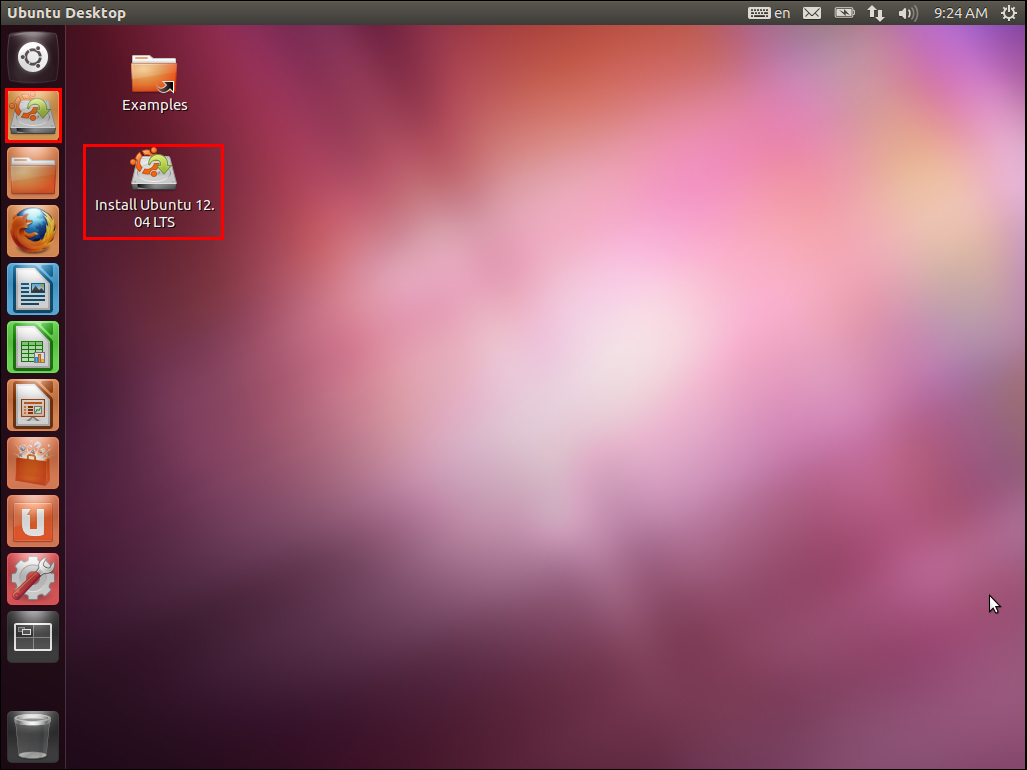
\includegraphics[width=400pt]{./images/installation/install-live1.png}
	\caption{Ubuntu Desktop}	
	\label{fig:live-desktop}	
	\end{center}
\end{figure}

\newpage
\section{Ubuntu as the only OS on the disk} \label{sect:ubuntu-install}
In the previous sections you read about how to run Ubuntu's live CD and what to do before you can actually install Ubuntu (e.g. backup your data, BIOS adjustment). Are you ready for the next step? If not, don't worry you can read the entire manual first, and when you are comfortable with everything you will be ready not just for the Ubuntu installation process but the usage too. If you are ready please be sure that you have done everything connected with steps before installation. If you haven't done everything, this is your last chance to do it before you go further. \\

\par \noindent As is mentioned earlier in this chapter, this section will describe how to install Ubuntu as the only operating system on your computer.This installation scenario is much easier than when considering to install Ubuntu alongside with Windows. All you have to be sure is that you have done the proper BIOS adjustment and backup of your data on to some external storage media like CD, DVD, USB or external disk.  \\

\par \noindent 1. Turn on the computer and insert the Ubuntu installation CD into the CD-ROM. Ensure that the BIOS is set to boot from the CD. Wait for the BIOS to read the CD and recognise the operating system. If everything is done properly you'll be able to see the Ubuntu start up screen as shown in figure \ref{fig:basic-start}.

\begin{figure}[h!]	
	\begin{center}
	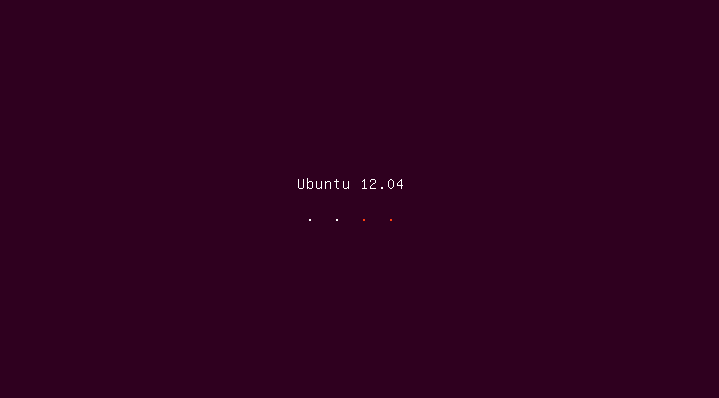
\includegraphics[width=300pt]{./images/installation/basic-start.png}
	\caption{Ubuntu start up screen}	
	\label{fig:basic-start}	
	\end{center}
\end{figure}

\par \noindent 2. Wait for Ubuntu to start up. Once the loading is complete, you are presented with the dialogue box as shown in figure \ref{fig:install-live-options} where you need choose to install Ubuntu. You can choose the installation language from the options shown on the left side.\\

\begin{figure}[!h]	
	\begin{center}
	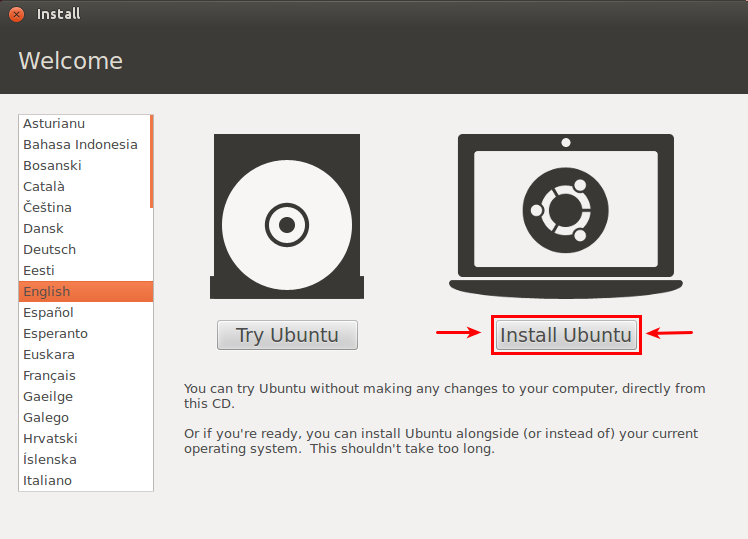
\includegraphics[width=300pt]{./images/installation/install-live-start2.png}
	\caption{Install Ubuntu option}	
	\label{fig:install-live-options}	
	\end{center}
\end{figure}

\par \noindent 3. Ubuntu checks if your system has access to the internet, connected to the power supply (laptop) and has atleast 4.4 Gb hard disk space. You will be also be required to choose If you want to install third party software and updates  during the installation. %Skip that part now because you can do that after you have installed it. 

\begin{figure}[!h]	
	\begin{center}
	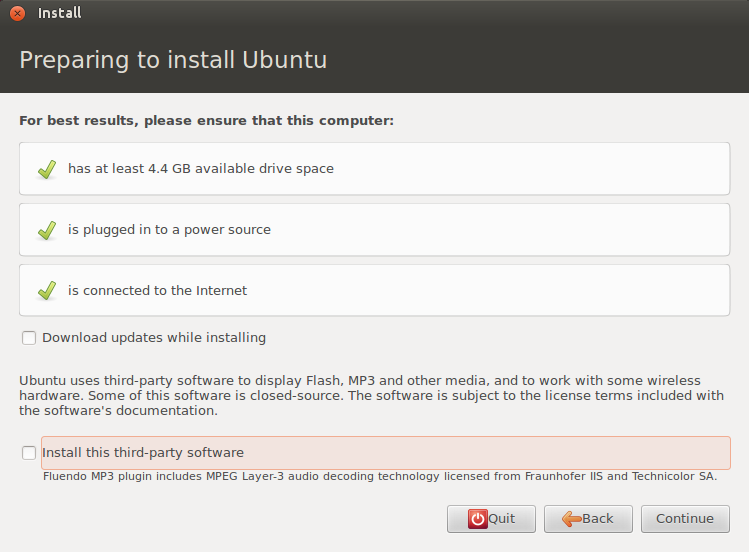
\includegraphics[width=300pt]{./images/installation/installer-prepare.png}
	\caption{Installer Options}	
	\label{fig:installer-prepares}	
	\end{center}
\end{figure}

\par \noindent 4. You are now presented with options to choose the type of installation you would like to perform. You can install Ubuntu alongside other operating systems (if you have any personal data, they will not be erased), Erase disk and install Ubuntu as the only operating system on your system or something else. If you have no other operating system installed on your system, then you will have only have the last two options. In this section which deals with Ubuntu as the only operating system, you need to choose the second option which removes any other operating system such as Windows XP, Vista or 7 and automatically does all the hard disk partitioning for you. \\

\begin{figure}[!h]	
	\begin{center}
	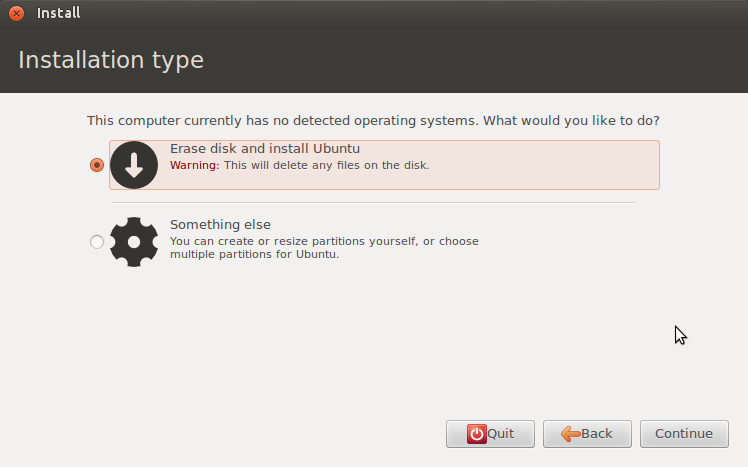
\includegraphics[width=300pt]{./images/installation/installer-os-options.png}
	\caption{Installer Options}	
	\label{fig:installer-prepare}	
	\end{center}
\end{figure}

\par \noindent On choosing the Erase disk and install Ubuntu option, you are presented with the following screen. Click on Install Now to start the Ubuntu installation. Note that this is permanent. If you click on Install Now, the installer erases all your data and installs Ubuntu! \\

\begin{figure}[!h]	
	\begin{center}
	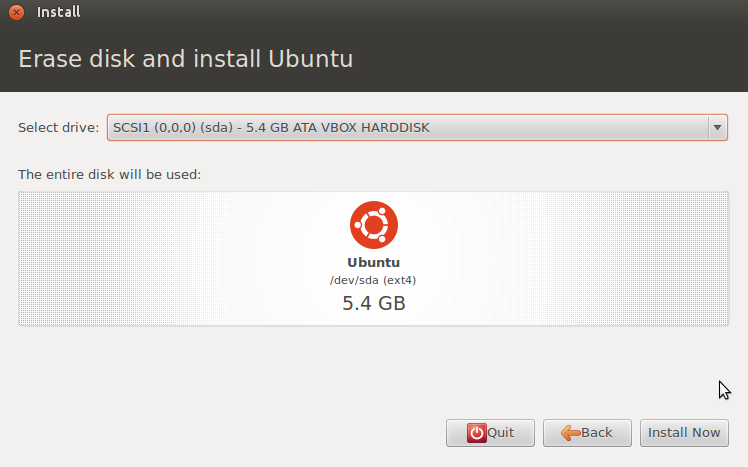
\includegraphics[width=300pt]{./images/installation/installer-onlyubuntu.png}
	\caption{Installer Options}	
	\label{fig:installer-onlyubuntu}	
	\end{center}
\end{figure}

\newpage
\par \noindent 5. The previous step was the hardest. Now it is basically entering some personal information. You first need to choose your keyboard layout. Ubuntu will automatically detect your keyboard layout. However, you can change the keyboard layout to match the local language settings. \\

\begin{figure}[!ht]	
	\begin{center}
	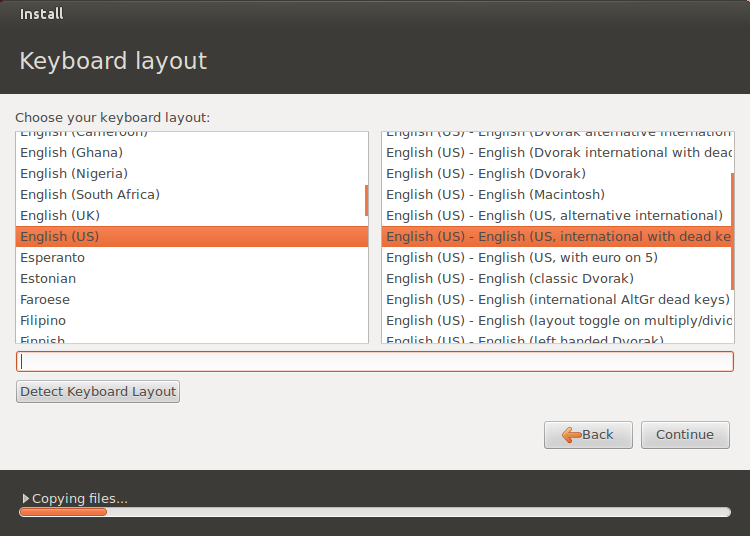
\includegraphics[width=300pt]{./images/installation/installer-keyboard.png}
	\caption{Installer Options}	
	\label{fig:installer-keyboard}	
	\end{center}
\end{figure}
\newpage
\par \noindent 6. You need to enter the place where you live. This is to automatically get the timezone and set the correct time. \\

\begin{figure}[!h]	
	\begin{center}
	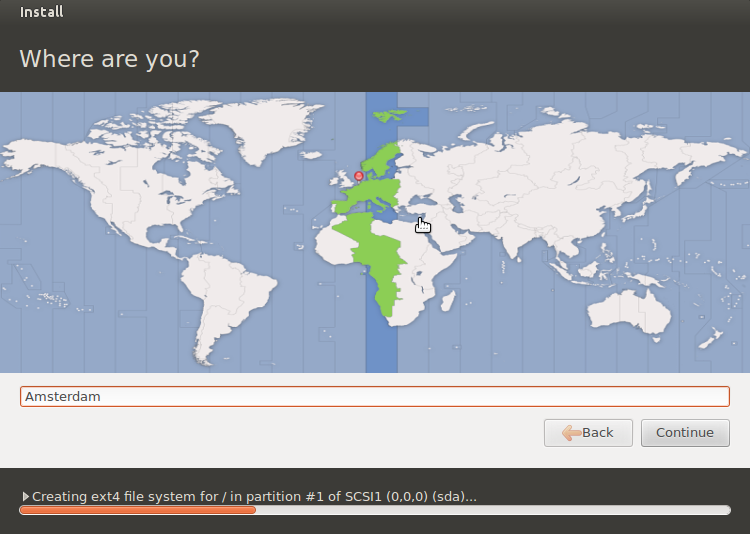
\includegraphics[width=300pt]{./images/installation/installer-timezone.png}
	\caption{Installer Options}	
	\label{fig:installer-keyboard}	
	\end{center}
\end{figure}

\par \noindent 7. The last step and this is where you set the username, password and other options like requiring a password to login in. \\

\begin{figure}[!h]	
	\begin{center}
	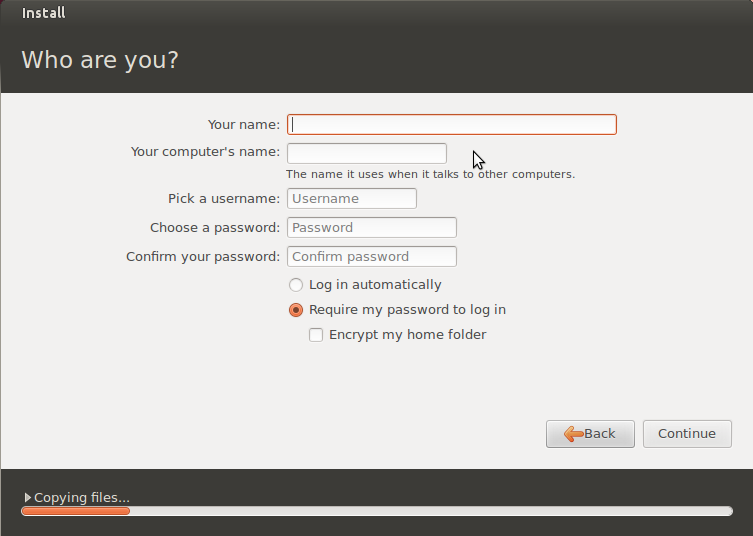
\includegraphics[width=300pt]{./images/installation/installer-who.png}
	\caption{Installer Options}	
	\label{fig:installer-who}	
	\end{center}
\end{figure}

\par \noindent After you have entered all the required data click on the button Continue and wait for around 20 minutes. After the installation is done, reboot your computer, take the CD out. The new operating system is waiting to be used. Congratulations on your Ubuntu install.

%\newpage
%\section{Ubuntu dual boot with Windows}
%It is not required to remove Windows to try out Ubuntu. You can have both of them install alongside each other to ease the transition to Ubuntu. In this section, the steps to dual boot Ubuntu with Windows are described. The Installation part remains pretty much the same with the only change in the disk partitioning and hence it is not necessary to show it all again. \\

%\par \noindent In this manual Windows XP is going to be used as a platform for making an example of the dual boot scenario. Partition Magic is the tool used to perform the partitioning . Do not worry if you do not have it. There are many alternatives for disk partitioning to choose from (e.g. GParted, Parted Magic). Ensure that you perform a backup of your data before proceed any further. \\

%\par \noindent On newer versions of Windows, you will not need an external program to make an extra partition. You can do that just by searching for disk partitioning in the start menu. You should now see the disk partitions on your system. So if you want to create a new partition under Windows 7, right click on the disk partition and choose Shrink unit command. However, in this section the partitioning will be shown with the Partition Magic 8.0 tool since Windows XP does not have this inbuilt. \\

%\par \noindent In figure \ref{fig:partitionmagic-main}, you will see the main interface of Partition Magic. In the figure, the partitioning is already done, but rest assured the steps will be shown.

%\begin{figure}[!h]	
%	\begin{center}
%	\includegraphics[width=300pt]{./images/installation/partitionmagic-main.png}
%	\caption{Installer Options}	
%	\label{fig:partitionmagic-main}	
%	\end{center}
%\end{figure}

\newpage
\section{Ubuntu on a virtual machine}
This section will describe how to try or install Ubuntu virtually without affecting your existing setup. By virtually running Ubuntu on a virtual machine, it is the same as you would use it if it was natively installed on your computer. Before proceeding, it is good to mention that you will need a spare 1 GiB of memory and atleast 8 GB of hard disk space. Then only can you actually run Ubuntu on a virtual machine. The virtually run Ubuntu is a guest operating system on your computer, and will use the same memory as your currently running operating system.  Hence you need memory for your current operating system plus memory for running Ubuntu. For instance, if you wanted to virtually run Ubuntu on a Windows Vista machine, you would need 2 GB (for Windows Vista) plus 1 GB (for Ubuntu) to use this method. For this example about how to setup a virtual machine, the application VirtualBox is used. You can  also use other alternatives namely, VMware, Parallels etc.  \\

\par \noindent 1. Open VirtualBox application, and left click on the New button as shown in figure \ref{fig:virtualbox-main} to start the virtual machine setup process. \\

\begin{figure}[!h]	
	\centering
	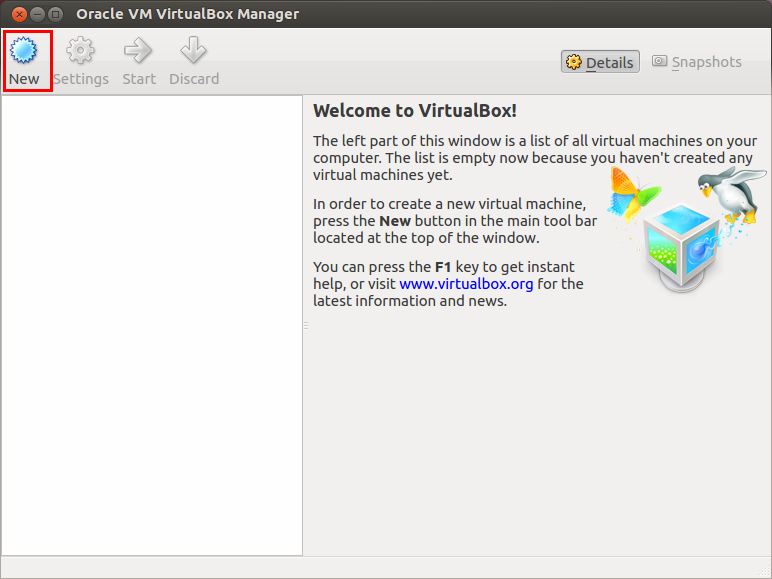
\includegraphics[width=300pt]{./images/installation/virtualbox/virtualbox-main.png}
	\caption{VirtualBox Manager main interface}	
	\label{fig:virtualbox-main}	
\end{figure}

\par \noindent 2. Type a virtual machine name. VirtualBox can automatically recognize the operating system you are going to use or install using the name. So if you type Ubuntu 12.04 LTS, VirtualBox will automatically fill in Linux and Ubuntu in the second and third blank box as shown in figure \ref{fig:wizard-newvirtual}. \\

\begin{figure}[!h]	
	\centering
	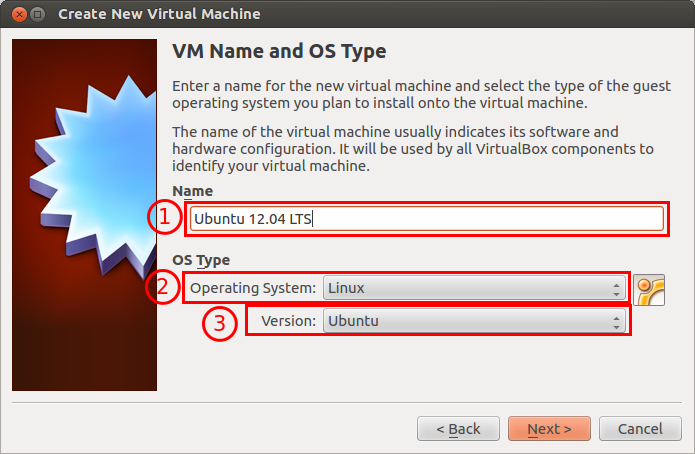
\includegraphics[width=300pt]{./images/installation/virtualbox/wizard-newvirtual.png}
	\caption{Virtual machine details}	
	\label{fig:wizard-newvirtual}	
\end{figure}

\par \noindent 3. Here you will have to give the guest operating system memory that it will use while running. It will use part of your memory that your current operating system already uses. It is recommended to atleast 512 MB (VirtualBox has already done that by default as seen in figure \ref{fig:wizard-memory}), but you can provide more if you have sufficient memory.  You will then just have to click on the button Next. \\

\begin{figure}[!h]	
	\centering
	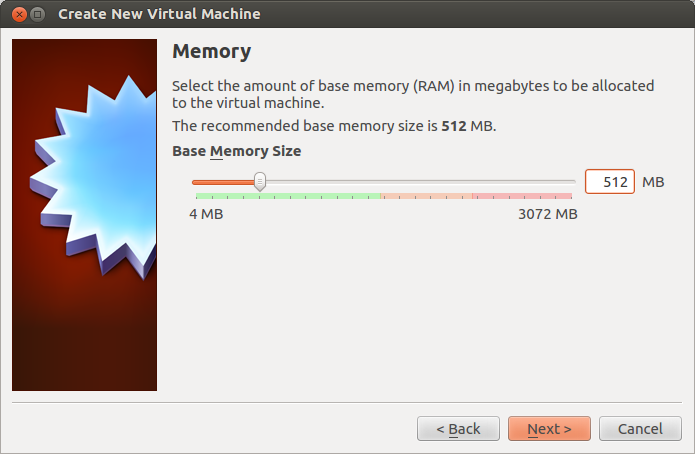
\includegraphics[width=300pt]{./images/installation/virtualbox/wizard-memory.png}
	\caption{Memory size for guest operating system}	
	\label{fig:wizard-memory}	
\end{figure}

\par \noindent 4. Here you will just have to give some disk space to the guest operating. The minimum recommended is 8 GB as you can see in figure \ref{fig:wizard-newharddisk}.  Remember the concept of a hard disk for the guest operating system is virtual. In reality, you will be basically creating a file of the size 8 GB. This will in no way affect your current hard disk partitions. \\ 

\begin{figure}[!h]	
	\centering
	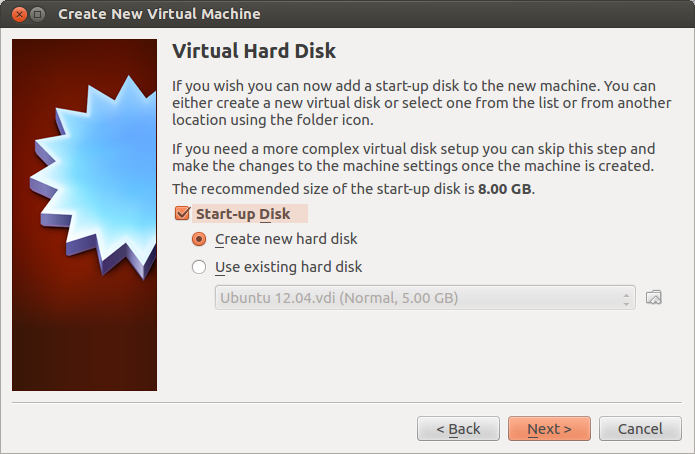
\includegraphics[width=300pt]{./images/installation/virtualbox/wizard-newharddisk.png}
	\caption{New startup disk}	
	\label{fig:wizard-newharddisk}	
\end{figure}

\par \noindent Click Next to proceed to create this file which will serve as a virtual hard disk for your guest operating system. Based on your disk space you can give it any value more than 8 GB.\\

\newpage
\par \noindent 5. In this step you will only have to choose the VirtualBox disk image and nothing else. VirtualBox does that already by the default as seen in figure \ref{fig:wizard-VDI}. \\

\begin{figure}[!h]	
	\centering
	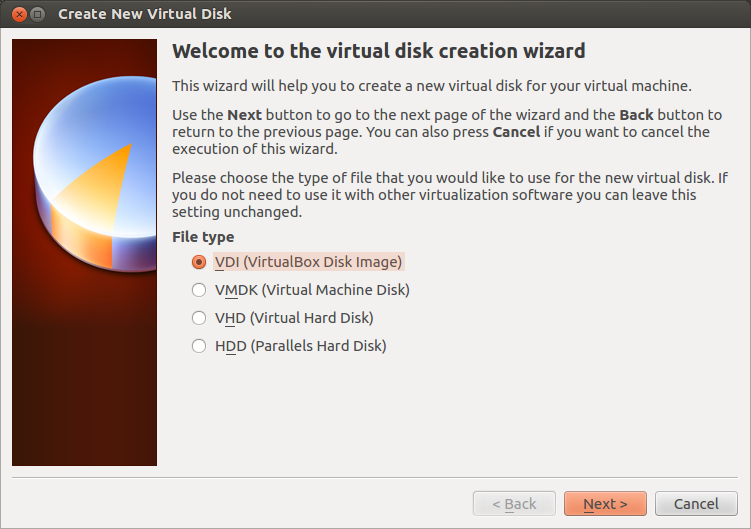
\includegraphics[width=300pt]{./images/installation/virtualbox/wizard-VDI.png}
	\caption{VirtualBox disk image}	
	\label{fig:wizard-VDI}	
\end{figure}

\par \noindent 6. Here you can choose to set the property of the new virtual disk. The virtual disk size can be dynamically allocated  or have a fixed size. Choose dynamically allocated as shown in figure \ref{fig:wizard-dynamicsize}. If you will use the new guest operating system for a while, there is a possibility that you will need space for new applications and the disk space required might grow. By choosing dynamically allocated size, you won't have to worry that your virtual machine might end up with lack of space. It will grow dynamically as the operating system grows. \\

\begin{figure}[!h]	
	\centering
	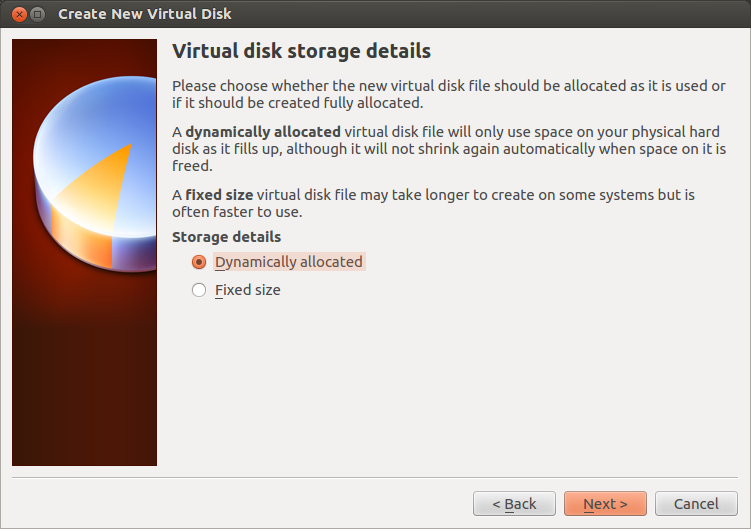
\includegraphics[width=300pt]{./images/installation/virtualbox/wizard-dynamicsize.png}
	\caption{VirtualBox disk storage details}	
	\label{fig:wizard-dynamicsize}	
\end{figure}

\newpage
\par \noindent 7. As seen in figure \ref{fig:wizard-newharddisk}, the minimum disk size for the guest operating system is 8 GB. As shown in figure \ref{fig:wizard-sizelocation}, you can set the virtual disk size from 8GB or more.  It actually depends on how much disk space you have at all.  \\

\begin{figure}[!h]	
	\centering
	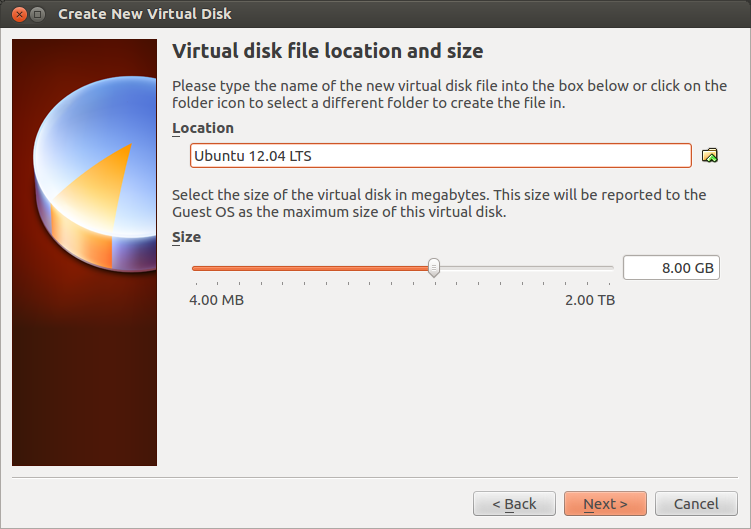
\includegraphics[width=300pt]{./images/installation/virtualbox/wizard-sizelocation.png}
	\caption{VirtualBox disk storage details}	
	\label{fig:wizard-sizelocation}	
\end{figure}

\par \noindent 8. Press Create to finish the wizard. You have now successfully created a virtual machine for running Ubuntu 12.04 LTS. With this you have created a virtual machine, but you still need to configure it and then actually perform the Ubuntu installation on the virtual hard disk.\\

\begin{figure}[!h]	
	\centering
	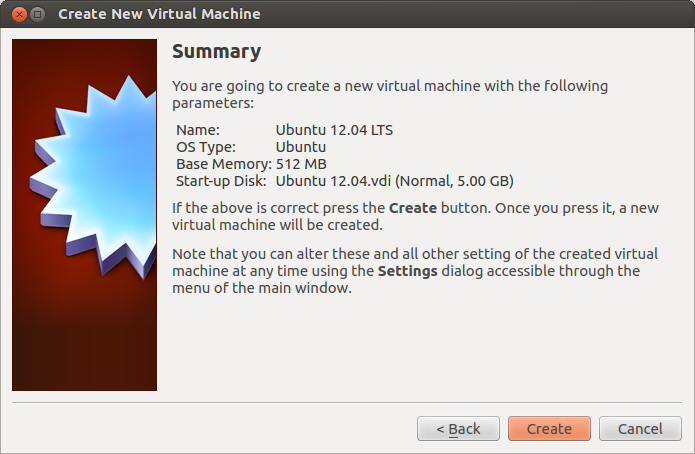
\includegraphics[width=300pt]{./images/installation/virtualbox/Wizard-complete.png}
	\caption{Wizard complete}	
	\label{fig:Wizard-complete}	
\end{figure}

\newpage
\par \noindent 9. With the wizard complete, you now need to configure the virtual machine before you can use it. This is illustrated below. Open the setting dialog by clicking the settings button as shown in figure \ref{fig:wizard-final}. \\

\begin{figure}[!h]	
	\centering
	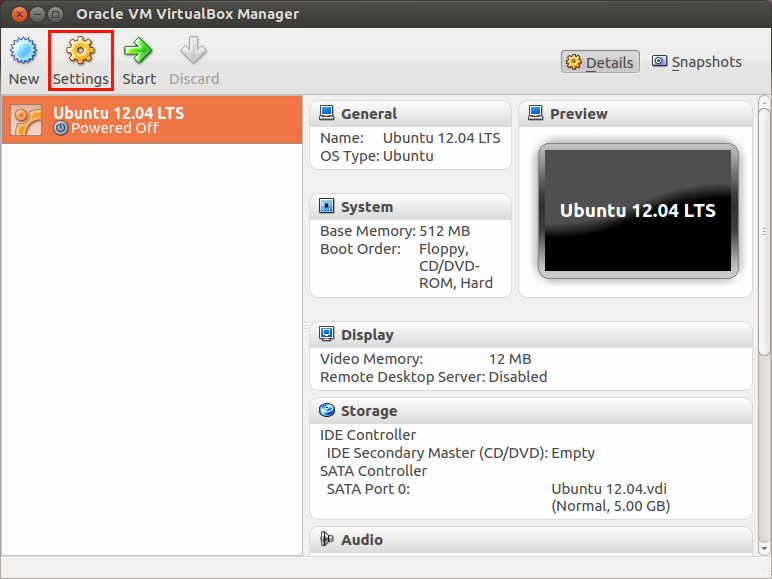
\includegraphics[width=300pt]{./images/installation/virtualbox/wizard-final.png}
	\caption{Click settings button}	
	\label{fig:wizard-final}	
\end{figure}

\par \noindent 10. Here you can adjust general stuff like virtual machine name to advanced things like sharing folders between your virtual operating system and natively installed operating system. The main focus here however is to change the display settings. First set the video memory to a value where Ubuntu can run reasonably well on your virtual machine. You could set it 128 MB or more preferable for better performance. Second, enable 3D acceleration. This is required to run Unity. You can see the steps illustrated in figure \ref{fig:settings-display}. \\

\begin{figure}[!h]	
	\centering
	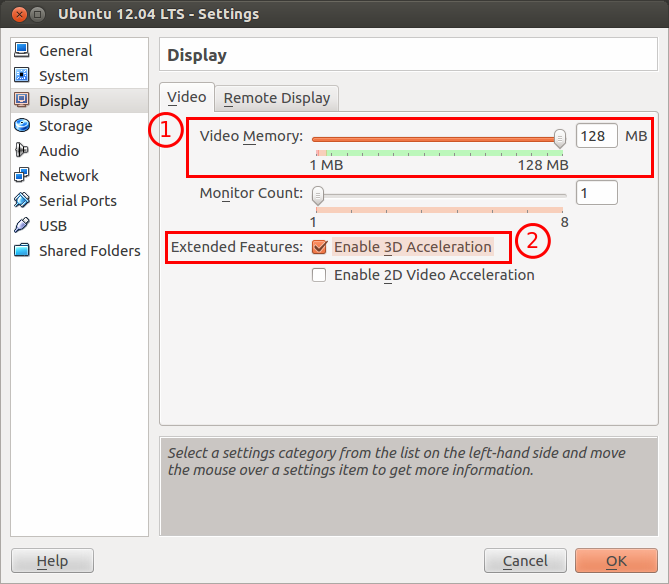
\includegraphics[width=300pt]{./images/installation/virtualbox/settings-display.png}
	\caption{Display settings}	
	\label{fig:settings-display}	
\end{figure}

\par \noindent 11. Finally, you need to provide the installation medium (in this case the Ubuntu ISO file) so that the virtual machine will try to install Ubuntu from this file. You can select the ISO file by clicking on the CD icon shown in 2nd box in figure \ref{fig:settings-storage}. \\

\begin{figure}[!h]	
	\centering
	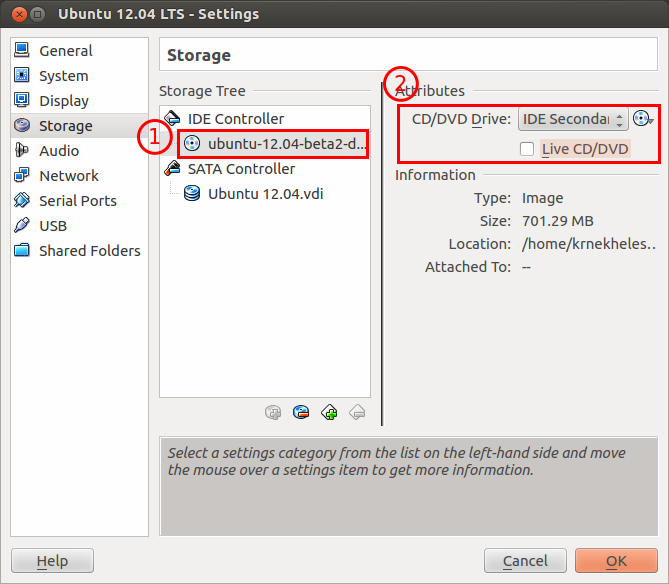
\includegraphics[width=300pt]{./images/installation/virtualbox/settings-storage.png}
	\caption{ISO File path}	
	\label{fig:settings-storage}	
\end{figure}

\par \noindent And that's it. You have completed configuring the virtual machine. Now close the settings dialog and click on the start button. The virtual machine will now open and you can proceed to install Ubuntu on the virtual hard disk from there. The entire Ubuntu installation process is already covered in section \ref{sect:ubuntu-install}. \\




